
% $Header: /cvsroot/latex-beamer/latex-beamer/solutions/generic-talks/generic-ornate-15min-45min.en.tex,v 1.5 2007/01/28 20:48:23 tantau Exp $

\documentclass[smaller]{beamer}
\mode<presentation>
{
  \usetheme{Singapore}
  \usefonttheme[onlymath]{serif}
  % or ...
 %  \setbeamercovered{transparent}
  % or whatever (possibly just delete it)
}


\usepackage[czech]{babel}
% or whatever
\usepackage[utf8]{inputenc}
% or whatever
%\usepackage{times}
%\usepackage[T1]{fontenc}
% Or whatever. Note that the encoding and the font should match. If T1
% does not look nice, try deleting the line with the fontenc.


\title{PAS04 - Important discrete and continuous distributions}

\author{Jan B\v rezina}
\institute % (optional, but mostly needed)
{
  %\inst{2}%
  Technical University of Liberec
}


% If you wish to uncover everything in a step-wise fashion, uncomment
% the following command: 

%\beamerdefaultoverlayspecification{<+->}

% ***************************************** SYMBOLS
\def\div{{\rm div}}
\def\Lapl{\Delta}
\def\grad{\nabla}
\def\supp{{\rm supp}}
\def\dist{{\rm dist}}
%\def\chset{\mathbbm{1}}
\def\chset{1}

\def\Tr{{\rm Tr}}
\def\sgn{{\rm sgn}}
\def\to{\rightarrow}
\def\weakto{\rightharpoonup}
\def\imbed{\hookrightarrow}
\def\cimbed{\subset\subset}
\def\range{{\mathcal R}}
\def\leprox{\lesssim}
\def\argdot{{\hspace{0.18em}\cdot\hspace{0.18em}}}
\def\Distr{{\mathcal D}}
\def\calK{{\mathcal K}}
\def\FromTo{|\rightarrow}
\def\convol{\star}
\def\impl{\Rightarrow}
\DeclareMathOperator*{\esslim}{esslim}
\DeclareMathOperator*{\esssup}{ess\,sup}
\DeclareMathOperator{\ess}{ess}
\DeclareMathOperator{\osc}{osc}
\DeclareMathOperator{\curl}{curl}

%\def\Ess{{\rm ess}}
%\def\Exp{{\rm exp}}
%\def\Implies{\Longrightarrow}
%\def\Equiv{\Longleftrightarrow}
% ****************************************** GENERAL MATH NOTATION
\def\Real{{\rm\bf R}}
\def\Rd{{{\rm\bf R}^{\rm 3}}}
\def\RN{{{\rm\bf R}^N}}
\def\D{{\mathbb D}}
\def\Nnum{{\mathbb N}}
\def\Measures{{\mathcal M}}
\def\d{\,{\rm d}}               % differential
\def\sdodt{\genfrac{}{}{}{1}{\rm d}{{\rm d}t}}
\def\dodt{\genfrac{}{}{}{}{\rm d}{{\rm d}t}}

\def\vc#1{\mathbf{\boldsymbol{#1}}}     % vector
\def\tn#1{{\mathbb{#1}}}    % tensor
\def\abs#1{\lvert#1\rvert}
\def\Abs#1{\bigl\lvert#1\bigr\rvert}
\def\bigabs#1{\bigl\lvert#1\bigr\rvert}
\def\Bigabs#1{\Big\lvert#1\Big\rvert}
\def\ABS#1{\left\lvert#1\right\rvert}
\def\norm#1{\bigl\Vert#1\bigr\Vert} %norm
\def\close#1{\overline{#1}}
\def\inter#1{#1^\circ}
\def\ol#1{\overline{#1}}
\def\ul#1{\underline{#1}}
\def\eqdef{\mathrel{\mathop:}=}     % defining equivalence
\def\where{\,|\,}                    % "where" separator in set's defs
\def\timeD#1{\dot{\overline{{#1}}}}

% ******************************************* USEFULL MACROS
\def\RomanEnum{\renewcommand{\labelenumi}{\rm (\roman{enumi})}}   % enumerate by roman numbers
\def\rf#1{(\ref{#1})}                                             % ref. shortcut
\def\prtl{\partial}                                        % partial deriv.
\def\Names#1{{\scshape #1}}
\def\rem#1{{\parskip=0cm\par!! {\sl\small #1} !!}}

\def\Xint#1{\mathchoice
{\XXint\displaystyle\textstyle{#1}}%
{\XXint\textstyle\scriptstyle{#1}}%
{\XXint\scriptstyle\scriptscriptstyle{#1}}%
{\XXint\scriptscriptstyle\scriptscriptstyle{#1}}%
\!\int}
\def\XXint#1#2#3{{\setbox0=\hbox{$#1{#2#3}{\int}$}
\vcenter{\hbox{$#2#3$}}\kern-.5\wd0}}
\def\ddashint{\Xint=}
\def\dashint{\Xint-}

% ******************************************* DOCUMENT NOTATIONS
% document specific
\def\rh{\varrho}
\def\vl{{\vc{u}}}
\def\th{\vartheta}
\def\vx{\vc{x}}
\def\vX{\vc{X}}
\def\vr{\vc{r}}
\def\veta{\vc{\eta}}
\def\dx{\,\d\vx}
\def\dt{\,\d t}
\def\bulk{\zeta}
\def\cS{\close{S}}
\def\eps{\varepsilon}
\def\phi{\varphi}
\def\Bog{{\mathcal B}}
\def\Riesz{{\mathcal R}}
\def\distr{\mathcal D}
\def\Item{$\bullet$}

\def\MEtst{\mathcal T}
%***************************************************************************
% highlight color
\setbeamercolor{my blue}{fg=blue}
\def\blue#1{{\usebeamercolor[fg]{my blue} #1}}

\setbeamercolor{my green}{fg=green}
\def\green#1{{\usebeamercolor[fg]{my green} #1}}

% color for term definition
\setbeamercolor{my orange}{fg=orange}
\def\df#1{{\usebeamercolor[fg]{my orange} #1}}
\def\xskip{{\vspace{2ex}}}

\def\cz#1{{\small (#1)}}

\begin{document}

\begin{frame}
  \titlepage
\end{frame}


\section{Common discrete distributions}

\begin{frame}{Bernoulli trials}
 Experiment with two possible outcomes:
\begin{itemize}
 \item yes/no questions
 \item throwing coin
 \item born girl/boy
 \item defect on product
 \item test of quality
 \item \df{success}/\df{failure}
\end{itemize}

The probability of success is $p$.
\end{frame}


\begin{frame}{Bernoulli/Alternative $Alt(p)$}
\blue{description}: value $1$ with probability $p$, value $0$ with prob. $1-p$\\

\xskip
\blue{values:} $0, 1$\\
\blue{parameter:} probability $p$

\xskip
$P( X=1 ) = p$\\
$EX = 1p+0(1-p) = p$\\
$DX = (1-p)^2 p + (0 - p)^2 (1-p)=p(1-p)$
\end{frame}

\begin{frame}[fragile]{Binomial $Bi(n,p)$}
\blue{description:} number of successes in $n$ independent trials\\
\blue{example:} $k$ defects on $n$ products; selection with replacement (non-destructive)

\xskip
\blue{values:} $0, \dots, n$ \\
\blue{parameters:} probability $p$, number of trials $n$

\xskip
\[
 P(X=k) = \binom{n}{k}p^k(1-p)^{n-k};\quad 0\le k \le n
\]
$EX = np$ (calculation with shifting)\\
$DX = np(1-p)$

\xskip
Notes:\
$Alt(p) = Bi(1,p)$\\
\verb'R> plot( dbinom(0:n, n, p) )'
\end{frame}

\begin{frame}[fragile]{Hypergeometric $H(N,M,n)$}
\blue{description}:  number of successes in $n$ draws from a set of size $N$ containing $M$ successes without replacement
\\
\blue{description}: $k$ cracked eggs in $n$ drawn if there is $M$ cracked and $N$ total in the basket,\\
quality tests, destructive tests

\xskip
\blue{values}: $\max(0, n+M-N), \dots, \min(M,n)$ \\
\blue{parameters}: number drawn $n$, total $N$, total of successes $M$

\[
 P(X=k) = \frac{\text{$n$-draw has $k$ successes}}{\text{all $n$-draw}}=
  \binom{M}{k}\binom{N-M}{n-k}\binom{N}{n}^{-1}
\]

$EX = \frac{nM}{N}$\\
$DX = \frac{nM}{N}\big(1-\frac{M}{N}\big)\big(\frac{N-n}{N-1}\big)$

\xskip
Notes:
$H(N,M,n) \approx Bi(n,M/N)$ for big values $N/n$\\
\verb'R> plot( dhyper( 0:n, M, N-M, n) )'
\end{frame}

\begin{frame}{Geometric $G(p)$}
\blue{description}: number of trials until first success (included)\\
\blue{example}: number of production cycles until defect

\xskip
\blue{values}: $1, \dots, \infty$ \\
\blue{parameter}: probability of success $p$

\xskip
\[
 P(X=k) = (1-p)^{k-1}p
\]
$EX = \frac{1}{p}$\\
$DX = \frac{1-p}{p^2}$\\
\end{frame}

\begin{frame}{Negative binomial $NB(k,p)$}
\blue{description}: number of trials until $k$ successes (included)\\

\xskip
\blue{values}: $k, \dots, \infty$ \\
\blue{parameters}: probability of success $p$, number of successes $k$

\xskip
\[
 P(X=n) = \binom{n-1}{k-1}(1-p)^{n-k}p^k
\]
\dots last success is fixed, selecting $k-1$ successes from $n-1$ trials

\xskip
$EX = \frac{k}{p}$\\
$DX = \frac{k(1-p)}{p^2}$\\
$NB(k,p)$ is sum of $k$ RV $G(p)$
\end{frame}

\begin{frame}{Example}
Oil company; geological study reveals: 0.2 chance to strike oil per well.\\
What is prob. that there will be 2 strikes out of 7 wells?\\
What is prob. that we need to drill 7 wells to gain 2 strikes?\\
What is prob. that we need to drill more then 5 wells to gain 2 strikes?
\end{frame}


\begin{frame}{Poisson distribution}

\df{Poisson process}: number of events during (time) interval, assuming that:
\begin{itemize}
 \item events are evenly distributed with density $\lambda$ events over time unit
 \item events are independent
\end{itemize}
\blue{Example}: number of nuclear decays over given time, number of defects on given length of fabric

\xskip
\blue{values}: $0,\dots,\infty$\\
\blue{parameters}: density $\lambda$, period $t$
\[
 P(X=k) = \frac{(\lambda t)^k e^{-\lambda t}}{k!}
\]
\end{frame}

\begin{frame}{Poisson distribution - derivation }

Divide interval $t$ to $n$ pieces, use $Bi(n, \lambda t/n)$ and pass to the limit:
\begin{multline*}
 p_k = \lim_{n\to\infty} \frac{n!}{k!(n-k)!}\Big(\frac{\lambda t}{n}\Big)^k\Big(1-\frac{\lambda t}{n}\Big)^{n-k} =\\
 =\frac{(\lambda t)^k}{k!}\underbrace{\frac{n!}{n^k(n-k)!}}_{\to 1} \underbrace{\Big(1+\frac{-\lambda t}{n}\Big)^n}_{\to exp(-\lambda t)}
  \underbrace{\Big(1-\frac{\lambda t}{n}\Big)^{-k}}_{\to 1} 
\end{multline*}
\end{frame}

\begin{frame}{\dots expectation and variance}
Using expansion for $\exp(\lambda t)$:
\[
  \sum_{k=0}^{\infty} \frac{(\lambda t)^k}{k!} e^{-\lambda t} = e^{-\lambda t} \sum_{k=0}^{\infty} \frac{(\lambda t)^k}{k!}  = e^{-\lambda t} e^{\lambda t} = 1
\]
similarly for expectation: 
\[
EX = \sum_{k=0}^{\infty} k \frac{(\lambda t)^k}{k!} e^{-\lambda t} =  \lambda t \sum_{k=0}^{\infty} \frac{(\lambda t)^{k-1}}{(k-1)!} e^{-\lambda t}=\lambda t
\]
\dots and variance:
\begin{multline*}
DX = \sum_{k=0}^{\infty} (k^2 - (EX)^2)p_k = \sum_{k=0}^{\infty} k(k-1)p_k + kp_k - (\lambda t)^2 p_k = \\
=(\lambda t)^2 +(\lambda t) - (\lambda t)^2 = \lambda t 
\end{multline*}
  
\end{frame}

\section{Continuous distributions}

\begin{frame}{Exponential distribution $E(\lambda)$}
$X$ is time between two events in Poisson process with density $\lambda$.\\
Time until failure.

\vspace{2ex}
Consider random variable $N_t \sim Po(\lambda, t)$.\\
Event $\{X \le t\}$ (time until next P. event is smaller then $t$ 
is identical with event $\{N_t \ge 1\}$ (there will be at least one P.event during time $t$).\\
\[
 F_X(t)=P(X\le t) = 1 - P(N_t < 1) = 1 - \frac{(\lambda t)^0 e^{-\lambda t}}{0!} = 1 - e^{-\lambda t}
\]
\[
  f_X(t) = \frac{d}{dt} F_X(t) = \lambda e^{-\lambda t}
\]
\dots we have to assume $t>0$.
\[
 EX = \int_0^\infty t\lambda e^{-\lambda t} \d t 
 = -\Big[te^{-\lambda t}\Big]_0^{\infty} + \int_0^\infty e^{-\lambda t}
 = \Big[\frac{e^{-\lambda t}}{-\lambda}\Big]_0^\infty=\frac{1}{\lambda}
\]
\[
 DX = \frac{1}{\lambda^2}
\]
\end{frame}

\begin{frame}{Exponential distribution ``is without memory''}
Time until failure is independent on the history:\\
Prob. of no failure until time $a+b$ under condition of no failure until time $a$\\
is same as prob. of no failure until time $b$
\begin{multline*}
 P(X > a+b | X>a) = \frac{1-F(a+b)}{1-F(a)} \\
= \frac{e^{-\lambda(a+b)}}{e^{-\lambda a}}= e^{-\lambda b} = 1 - F(b) = P(X>b)
\end{multline*}

\end{frame}


\begin{frame}{Erlang distribution $Erlang(k,\lambda)$}
$X$ is time until $k$-th event in Poisson process with density $\lambda$. 
Particular case of more general \blue{Gamma distribution} (even for non-integer $k$)
\[
 f_X(t)=\lambda e^{-\lambda t} \frac{(\lambda t)^{k-1}}{(k-1)!}
\]
\[
  F_X(t) = 1- e^{-\lambda t}\sum_{i=0}^{k-1} \frac{(\lambda t)^{i}}{i!}
\]
\[
 EX = \frac{k}{\lambda}
\]
\[
 DX = \frac{k}{\lambda^2}
\]

\end{frame}


\begin{frame}{Relation between Bernoulli and Poisson process}
 \begin{center}
 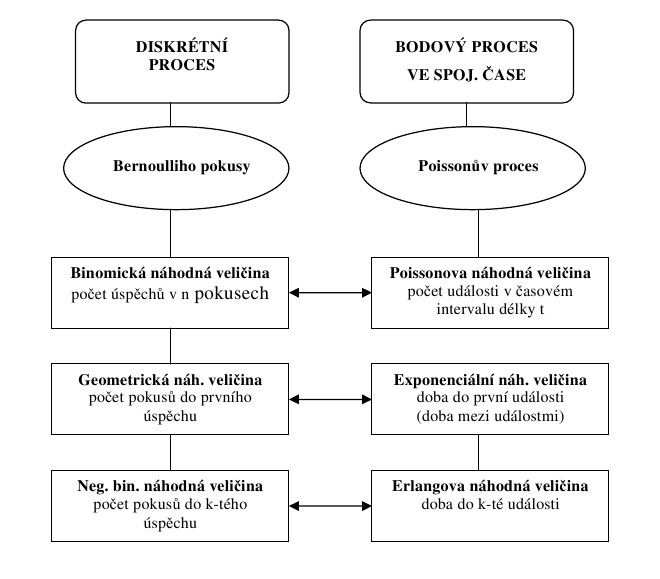
\includegraphics[scale=0.5]{./04_bernoulli_poisson.png}
 % bernoulli_poisson.png: 660x579 pixel, 96dpi, 17.46x15.32 cm, bb=0 0 495 434
\end{center}
\end{frame}


\begin{frame}{Uniform distribution $U(a,b)$}

\blue{density: }
\[f(x) = \left\{
   \begin{array}{l}
    \frac{1}{b-a}  \qquad \text{for }x\in[a,b]\\
     0 \qquad \text{elsewhere}
   \end{array}
\right.
\]

\blue{CDF: }
\[f(x) = \left\{
   \begin{array}{l}
    0 \qquad \text{pro } x< a\\
    \frac{x-a}{b-a}  \qquad \text{pro }x\in[a,b]\\
     1 \qquad \text{pro } x> b
   \end{array}
\right.
\]

\blue{mean value:}
\[
 EX = \int_a^b \frac{x}{b-a} \dx = \frac{1}{2(b-a)} \big(b^2 - a^2\big) = \frac{a+b}{2}
\]

\blue{variance:}
\[
 DX = \int_a^b \Big(\frac{a+b}{2} - x\Big)^2 \frac{1}{b-a} =\frac{(a-b)^2}{12}
\]
\end{frame}

\begin{frame}{Properties of uniform distribution.}
\begin{theorem}
For arbitrary RV $X$ with continuous increasing CDF $F_X$ the random variable 
\[
  Y=F_X(X)
\]
has uniform distribution $U(0,1)$. 
\end{theorem}
\blue{proof:} $P( Y \le y) = P( X \le F^{-1}_X(y))  = F_X( F^{-1}_X (y)) =y$

\xskip
Obviously it holds also in other direction:
\begin{theorem}
Let $Y \sim R(0,1)$ and $F$ is some distribution function, then $X = F_X^{-1}(Y)$ is random variable with CDF $F_X=F$.
\end{theorem}

\begin{itemize}
\item In the later theorem, $F$ can be arbitrary CDF (even discontinuous).
\item Computer generators of (pseudo)random numbers usually produce numbers with distribution $R(0,1)$.
\item The second theorem can be used to generate random numbers  with prescribed distribution. (approximation is used in practice)
\end{itemize}

\end{frame}



\begin{frame}[fragile]{Weibull distribution $W(\lambda, \beta)$}
Time until failure with shape/age parameter $\beta$.

\[
 F_X(t) = 1-exp\big( -(t/\lambda)^\beta \big )
\] 
\dots similar to exponential distribution.

\xskip
\blue{Meaning of parameter $\beta$}
\begin{itemize}
 \item  $k<1$ failure rate decreases over time, "infant mortality"
 \item  $k=1$ failure rate is constant over time, exponential distr.
 \item  $k>1$ failure rate increases with time, "aging" process
\end{itemize}

\verb'R> rweibull(n, beta, lambda)'
\end{frame}

\begin{frame}{Weibull distribution - influence of parameter $\beta$}
intensity of failures $\lambda(t) = f(t)/(1-F(t))$:
 \begin{center}
 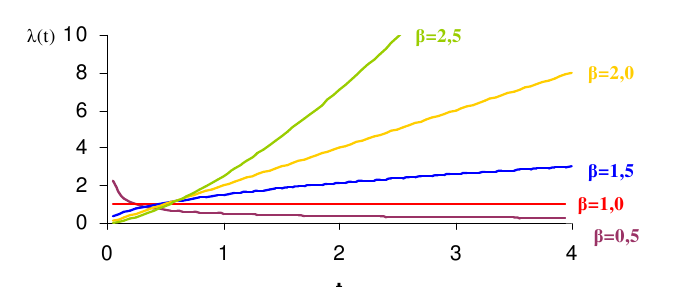
\includegraphics[scale=0.7]{./04_weibull_intenzita.png}
\end{center}
\end{frame}

\begin{frame}{Weibull distribution - influence of parameter $\beta$}
probability density function:
\begin{center}
 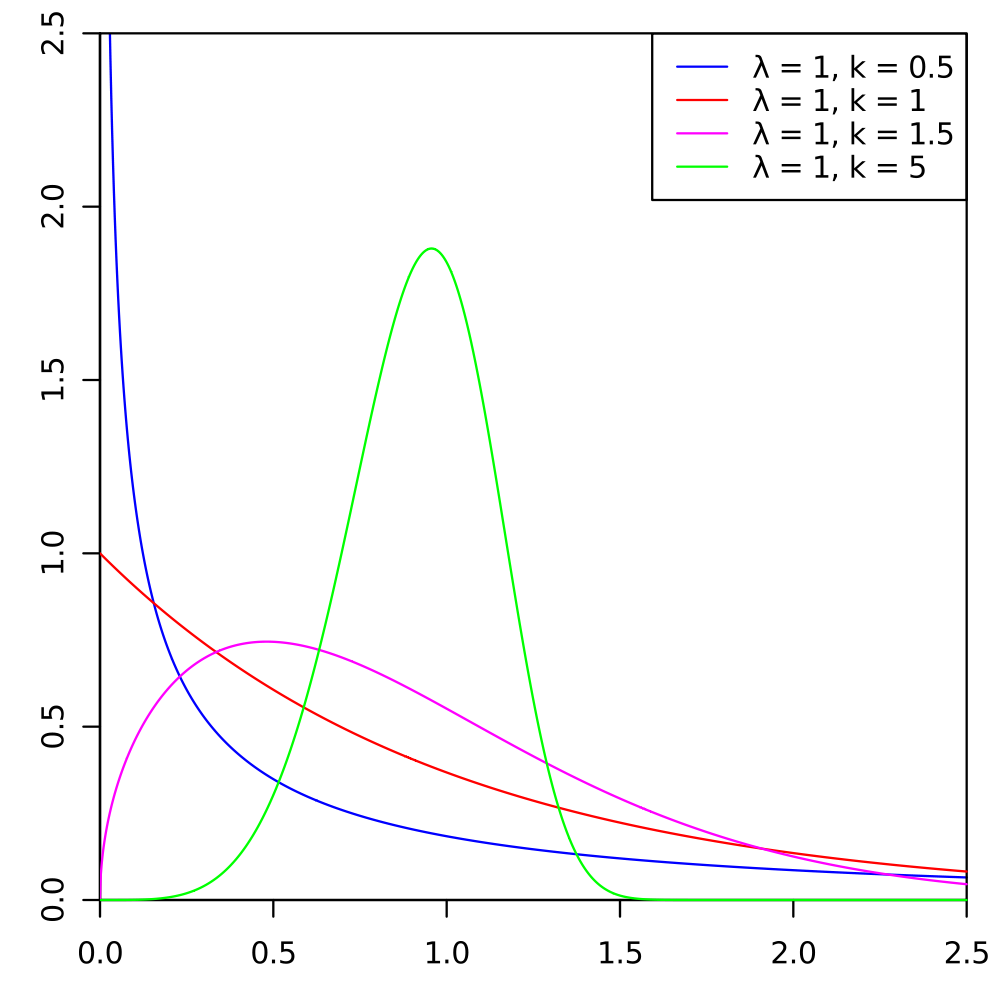
\includegraphics[scale=0.2]{./04_weibull_density.png}
\end{center}
\end{frame}

\begin{frame}{Normal distribution $N(\mu, \sigma^2)$}
Sum of large number of independent RV. Natural events. NOT social events.\\
density:
\[
 f(x) = \frac{1}{\sqrt{2\pi \sigma^2}} exp\Big( - \frac{ (x - \mu)^2}{2\sigma^2} \Big)
\]
CDF: $F(x) = errf(\frac{x-\mu}{\sigma})$ \dots integral of density, no closed formula\\
\vspace{2ex}
$EX = \mu$\\
$DX = \sigma^2$

\end{frame}

\begin{frame}{ND - density}
 \begin{center}
 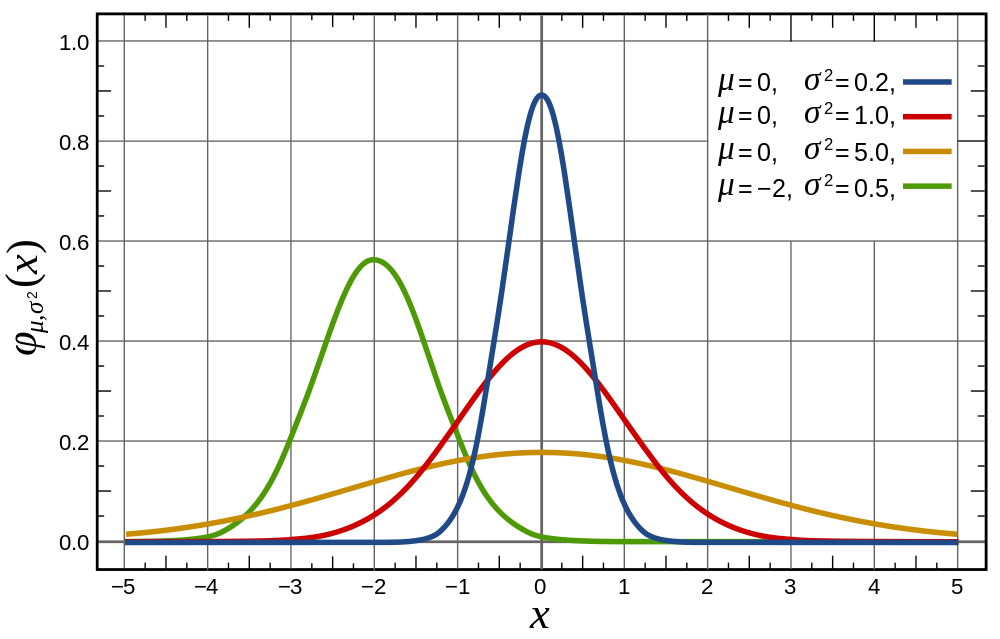
\includegraphics[scale=0.3]{./04_normal_distribution.png}
 % 04_normal_distribution.png: 1000x639 pixel, 72dpi, 35.28x22.54 cm, bb=0 0 1000 639
\end{center}

\end{frame}

\begin{frame}{Standard normal distribution $N(0,1)$}
Standardization of normal random variable $X \sim N(\mu, \sigma^2)$:
\[
 Y = \frac{X - \mu}{\sigma} \quad \sim N(0,1)
\]
and vice versa.
 \begin{center}
 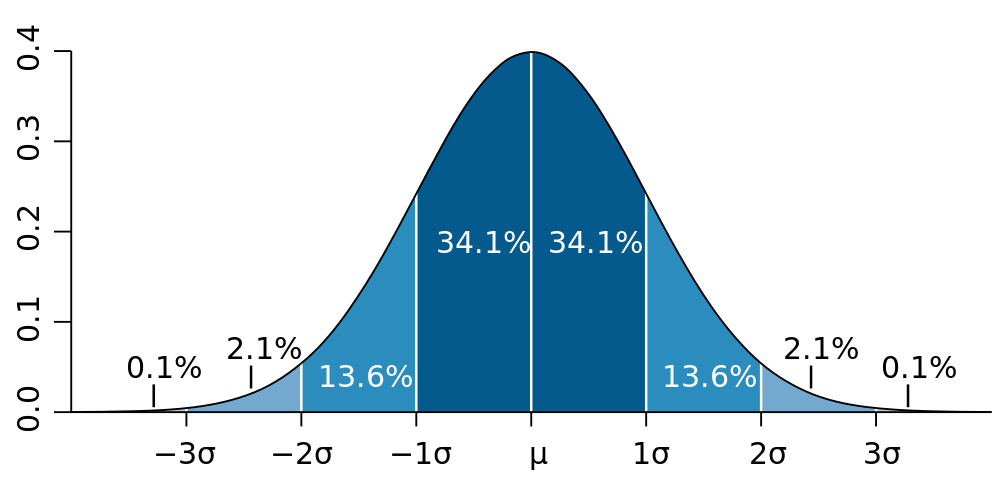
\includegraphics[scale=0.3]{./04_standard_deviation_diagram.png}
\end{center}

\end{frame}


\begin{frame}{Log-normal distribution $LN(\mu, \sigma^2)$}
$X$ is log-normal if $\ln X$ has normal distribution,
so $X=\exp( \mu + \sigma Z)$ where $Z \sim N(0,1)$.

density:
\[
 f(x) = \frac{1}{x\sqrt{2\pi \sigma^2}} exp\Big( - \frac{ (\ln\,x - \mu)^2}{2\sigma^2} \Big)
\]
\end{frame}

\begin{frame}{Presence of normality}
 When adding lot of random factors (central limit theorem):
 \begin{itemize}
  \item velocity of molecules
  \item measurements
  \item biological values (often log-norm, after separating male/female)
 \end{itemize}
\end{frame}




\end{document}


